Metro Extract

\section{Metro Extracts}

\subsection{pengertian Metro Extracts}
Metro Extracts adalah potongan data OpenStreetMap yang terpotong ke wilayah persegi panjang yang mengelilingi kota atau wilayah tertentu yang diminati. Ada ekstrak yang tersedia untuk diunduh langsung dari 200 wilayah paling populer dan Anda juga dapat membuat ekstrak khusus yang tersedia dalam 30-60 menit.
\begin{figure}[ht]
\centerline{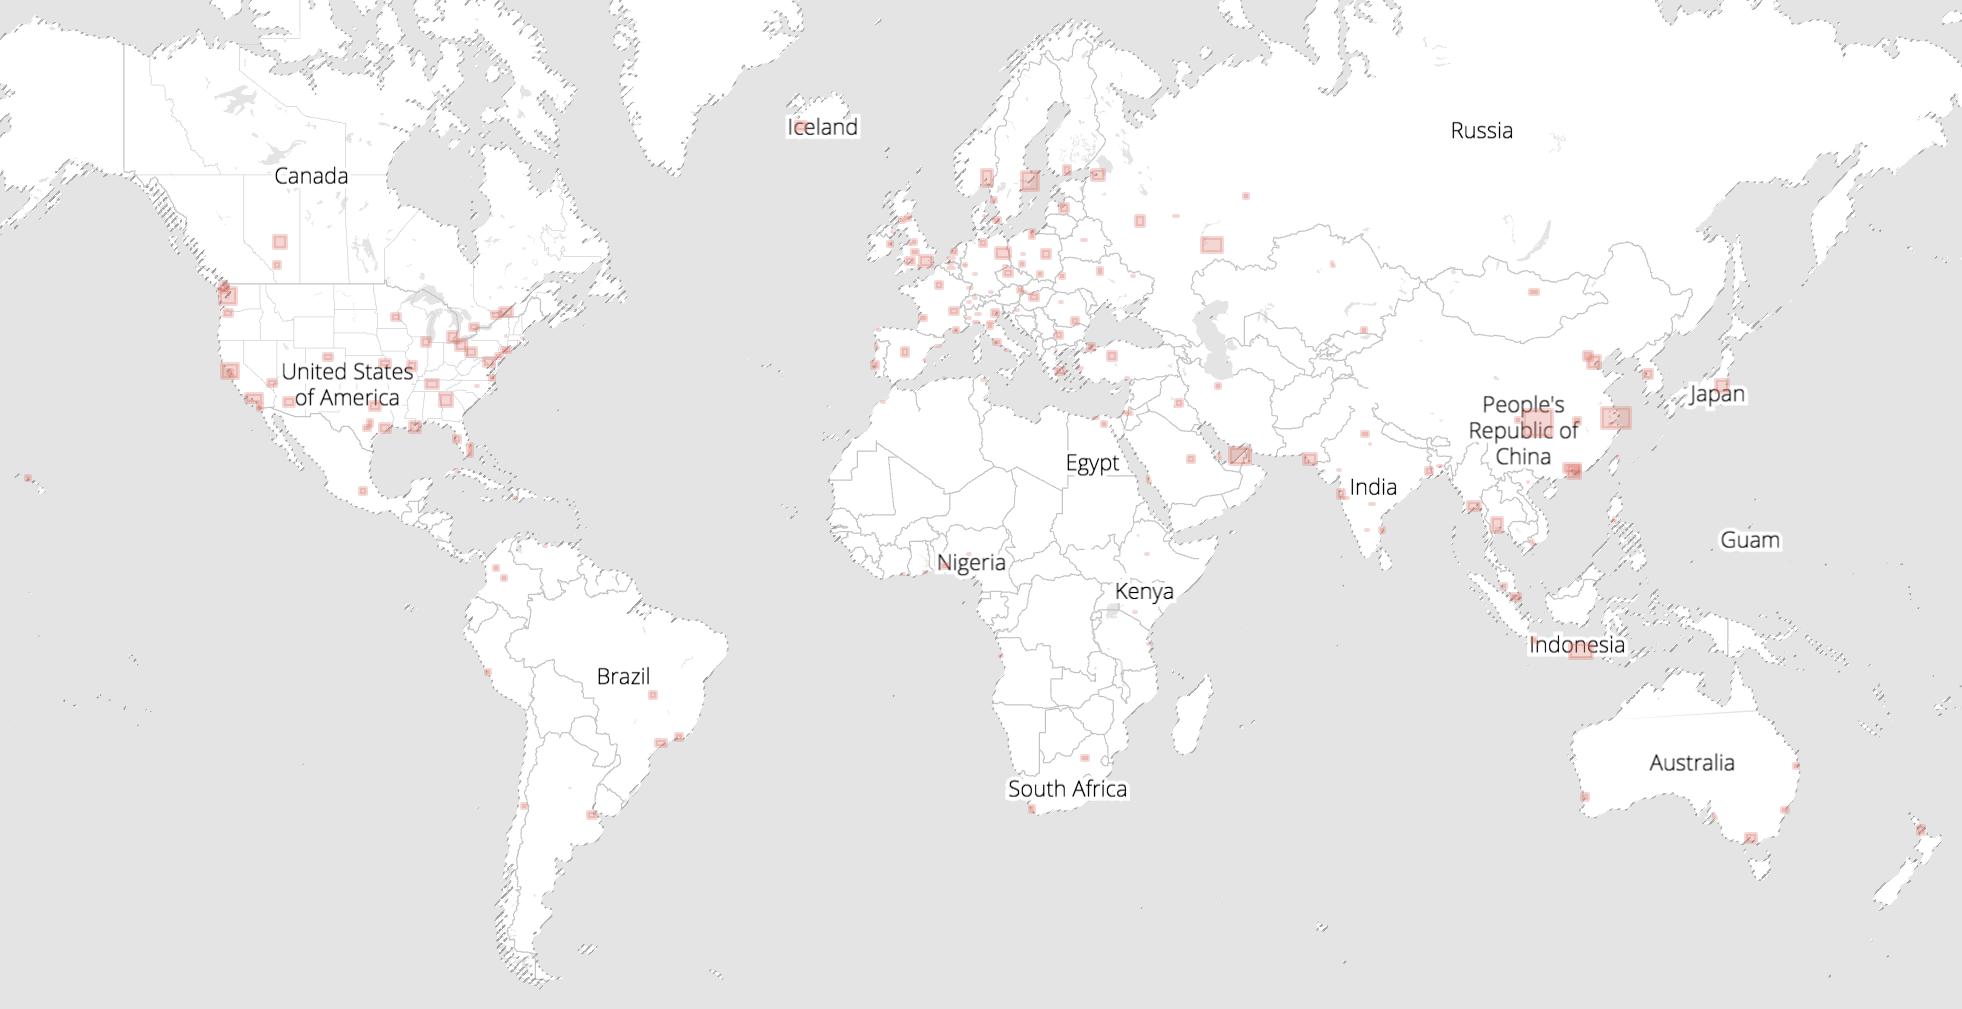
\includegraphics[width=0.25\textwidth]{figures/petadunia}}
\caption{gambar peta dunia}
\label {petadunia}
\end{figure}
Untuk mengunduh data OSM, buka laman unduhan Metro Extracts di https://mapzen.com/data/metro-extracts/ . Halaman ini memiliki peta web dan daftar tempat populer yang tersedia untuk diunduh langsung. Anda juga dapat membuat ekstrak khusus , yang membutuhkan waktu hingga 30-60 menit untuk dibuat dan memerlukan akun pengembang Mapzen gratis.
\subsection{Gunakan data Metro Extracts di QGIS}

Tutorial ini akan membahas cara mengunduh ekstrak data OSM untuk wilayah dan memuat file ke dalam QGIS , yang merupakan aplikasi GIS desktop open source gratis. Tercakup dalam tutorial ini adalah cara mendownload data dari Metro Extracts, format file mana yang akan dipilih, bagaimana cara membuka data di QGIS, dan bagaimana cara membuat peta Sydney, Australia. Anda bisa mengikuti dengan mendownload data untuk Sydney, atau memilih kota yang berbeda.
Untuk tutorial ini, kita akan melihat dua jenis format file yang cocok untuk alur kerja pemetaan khas di QGIS. Kedua jenis ini diproses ke berbagai tingkat granularitas yang dapat berguna untuk berbagai alasan. Satu jenis file memisahkan data OSM dengan tipe geometri, ini adalah ekstrak osm2pgsql .Yang lain, ekstrak imposm , sedikit lebih diproses dan memisahkan data OSM dengan berbagai tag, memisahkan data ke dalam lapisan logis seperti jalan, batas administratif, bangunan, dan sebagainya.
\subsection{Persyaratan}
\begin{enumerate}
\item 
Sambungan internet dengan kemampuan mendownload file Ekstrak Metro. Data Sydney yang digunakan dalam latihan ini sekitar 23 MB, namun unduhan untuk kota lain berkisar antara 2 MB sampai 350 MB.
\item
QGIS dan dependensinya, seperti GDAL. QGIS tersedia untuk berbagai platform, termasuk Windows dan Mac. Jika Anda perlu menginstal QGIS, ikuti petunjuk untuk sistem operasi Anda. Tutorial ditulis menggunakan QGIS 2.14 (Essen).
\end{enumerate}

\subsection{Download file ekstrak}
\begin{enumerate}
\item
Buka browser web ke halaman download Ekstrak Metro di https://mapzen.com/data/metro-extracts/ . Halaman memiliki peta yang menunjukkan download yang tersedia, serta kotak filter dan daftar nama kota di bawahnya.

\begin{figure}[ht]
\centerline{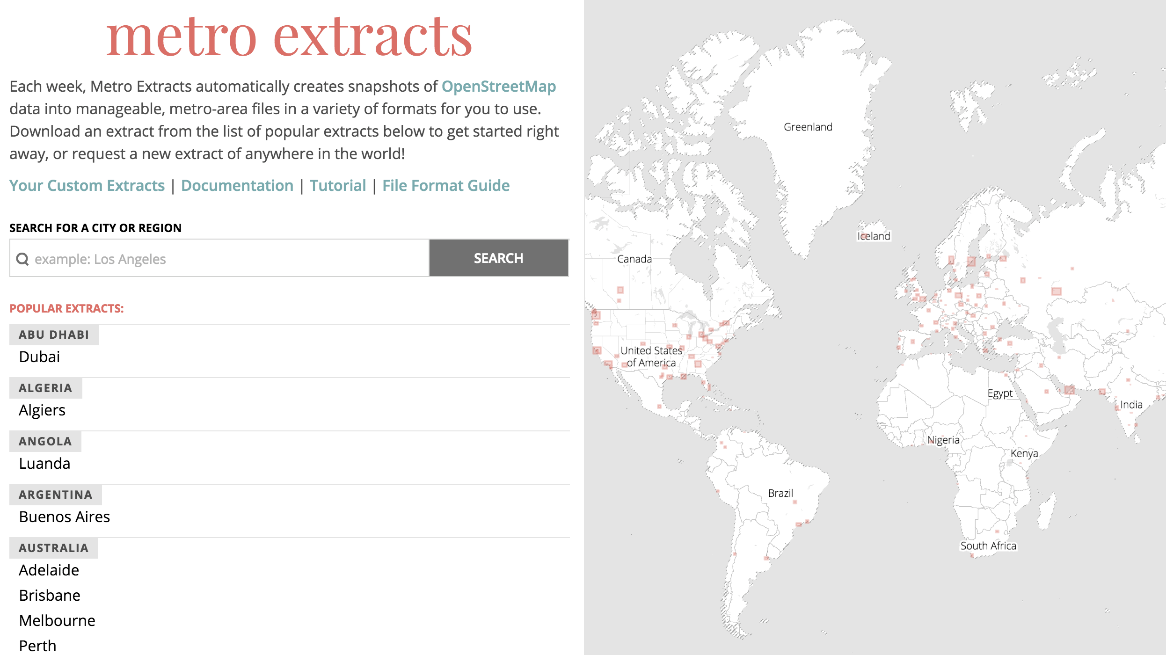
\includegraphics[width=0.25\textwidth]{figures/halamanawal}}
\caption{halaman awal pada metro extract}
\label {halamanawal}
\end{figure}

\item 
Bagian kiri halaman memiliki daftar 200 area ekstrak metro populer yang tersedia untuk diunduh langsung. Untuk tutorial ini, kita akan memilih Sydney, Australia yang masuk dalam daftar. Ekstrak khusus juga bisa dibuat.
\item
Untuk memilih Sydney, Anda dapat menggulir daftar sampai Anda melihat nama ekstrak (perhatikan bahwa mereka diatur menurut negara), gunakan bilah penelusuran, atau perbesar peta di sisi kanan halaman.Setelah Anda navigasikan ke ekstrak, klik 'Sydney' untuk memilih format file.
\item
Setelah memilih sebuah metro, Anda akan diarahkan ke halaman yang memungkinkan Anda melihat ekstrak di peta, dan memilih format file yang akan diunduh. Ada banyak format yang tersedia, tergantung pada apa yang ingin Anda gunakan untuk data ini. Pelajari lebih lanjut tentang format file di Metro Extracts.

\begin{figure}[ht]
\centerline{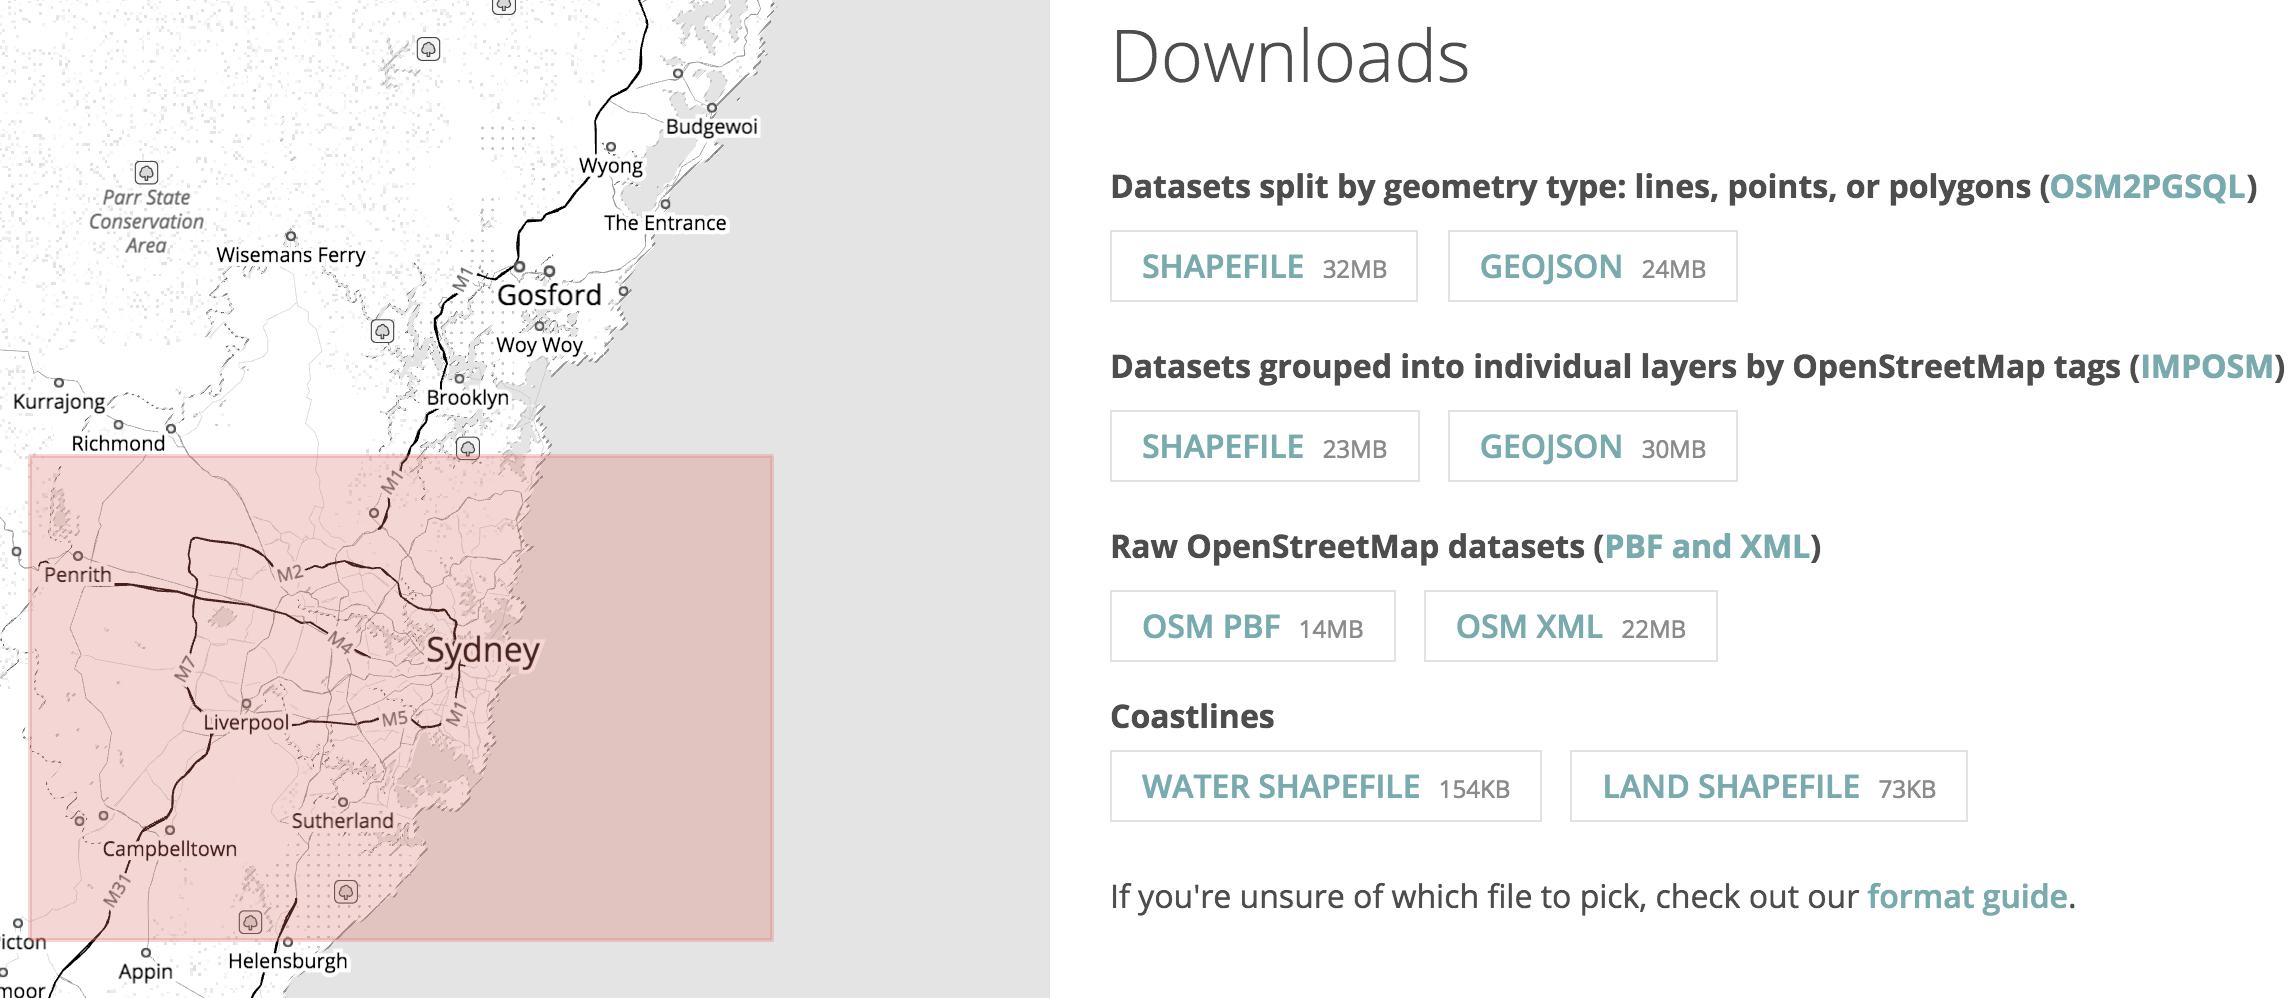
\includegraphics[width=0.25\textwidth]{figures/formatfile}}
\caption{download format file}
\label {formatfile}
\end{figure}


\item
Pilih salah satu dari masing-masing jenis data yang diproses (osm2pgsql dan imposm) pada halaman ekstrak. Masing-masing format file ini memiliki dua pilihan yang berbeda: GeoJSON atau Shapefile. Demi tutorial ini, kita akan menggunakan salah satu dari setiap pilihan untuk melihat perbedaan antara jenis ekstrak OSM yang berbeda serta format file data spasial yang berbeda.

\end{enumerate}

\subsection{Download format file}

\begin{figure}[ht]
\centerline{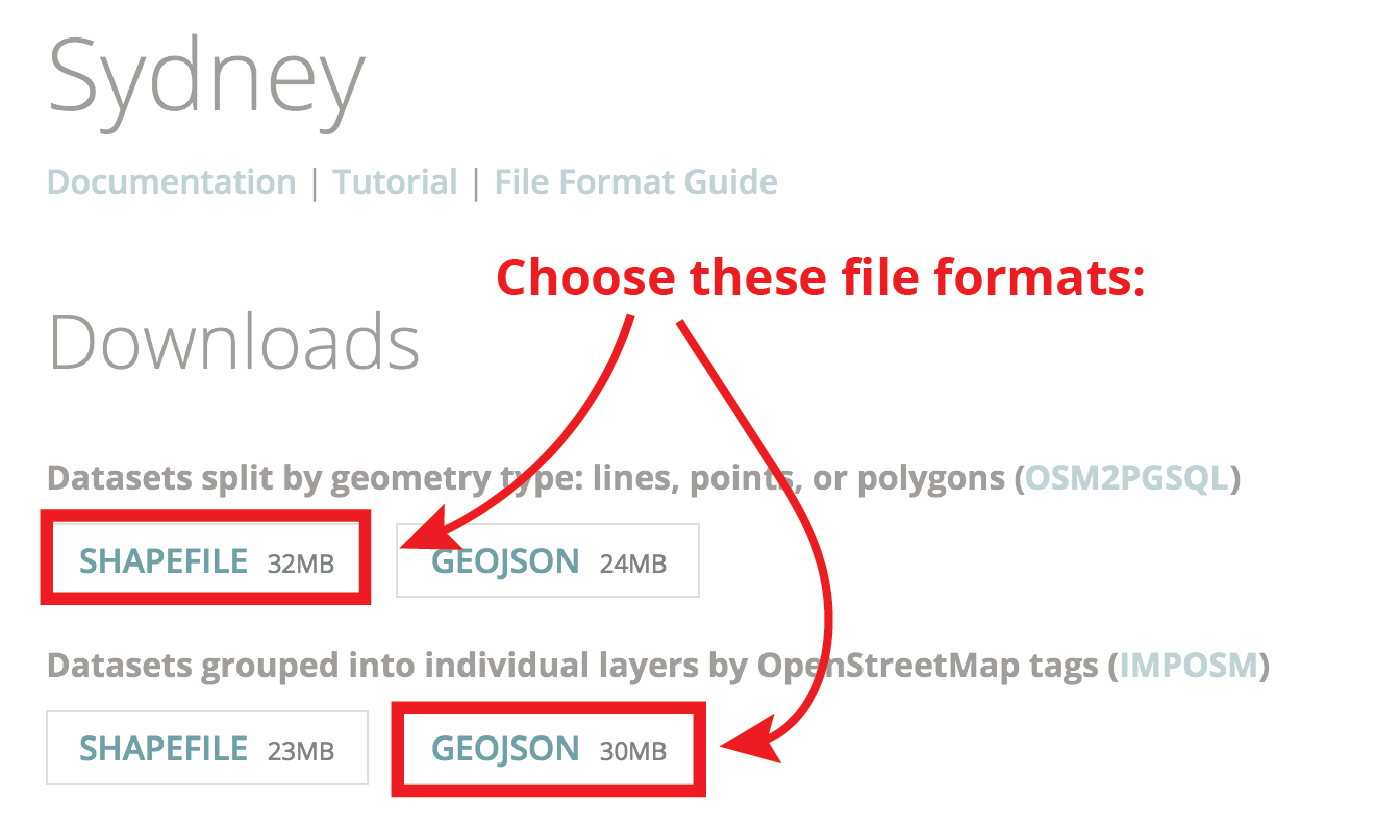
\includegraphics[width=0.25\textwidth]{figures/downloadfile}}
\caption{download filemap}
\label {downloadfile}
\end{figure}

\begin{enumerate}
\item
Di bawah judul OSM2PGSQL, klik tombol SHAPEFILE untuk mendownload file.
\item
Di bawah judul IMPOSM, klik tombol GeoJSON untuk mendownload file.
\item
Temukan file yang diunduh di disk (secara default, mereka akan berada di folder unduhan mesin Anda) dan unzip mereka jika tidak dibuka secara otomatis. Harus ada dua folder, masing-masing berisi file Metro Extracts yang sesuai.
\end{enumerate}
Catatan: Jika Anda menggunakan Safari sebagai browser Anda, unduhan Anda mungkin akan dibuka secara otomatis dan folder diberi nama sedikit berbeda dari yang ditunjukkan dalam tutorial ini.
Sementara GeoJSON adalah file tunggal .geojson pada disk, satu shapefile dibuat dari file individual (.shp, .dbf, .prj, dan seterusnya), jadi jangan hapus atau pindahkan secara terpisah salah satu dari file penyusun ini agar tidak merusak shapefile dan harus mendownloadnya lagi. Jika Anda mengelola file melalui perangkat lunak SIG, komponen diperlakukan sebagai keseluruhan entitas dan diperbarui dengan tepat.

\subsection{Tambahkan shapefile OSM2PGSQL ke QGIS}
Setelah file diunduh, Anda akan memasukkannya ke dalam QGIS.
\begin{enumerate}
\item
Mulai QGIS dan tampilkan peta kosong.
\item
Pada panel Browser, navigasikan ke folder download (atau dimanapun shapefile dan GeoJSON Anda didownload) dan buka folder 'sydney australia.osm2pgsql-shapefiles'. Jika Anda mendownload kota selain Sydney, navigasikan ke folder itu dan lebarkan isinya.
\item
Perhatikan bahwa folder berisi tiga shapefile, dinamai dengan tipe geometri: titik, garis, dan poligon.
\item
Klik dua kali pada layer line untuk membukanya di peta. Karena ekstrak didasarkan pada kotak pembatas persegi panjang, batas lapisan akan melampaui batas administratif sebenarnya dari sebuah kota.
\end{enumerate}

\begin{figure}[ht]
\centerline{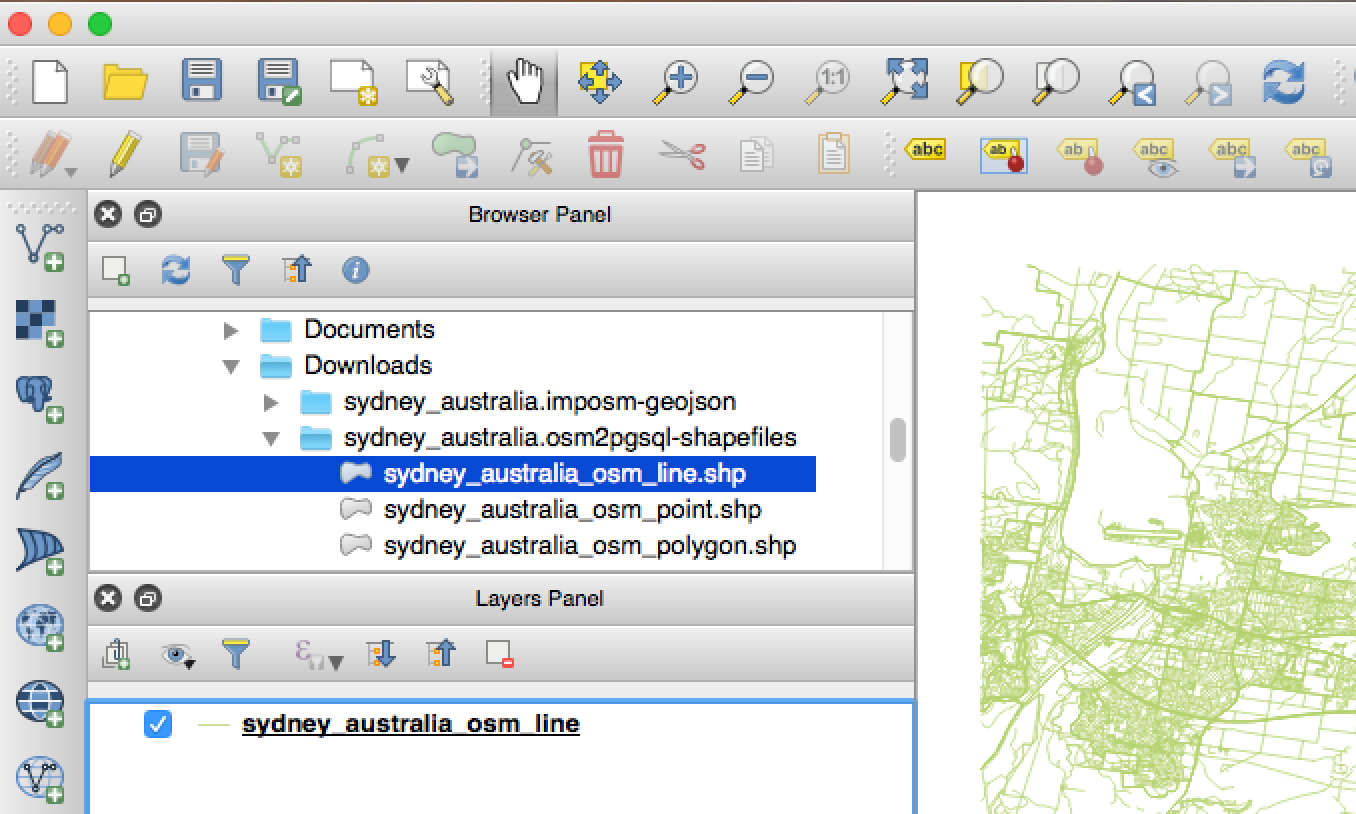
\includegraphics[width=0.25\textwidth]{figures/filepeta}}
\caption{gambar file peta}
\label {filepeta}
\end{figure}

\subsection{Tambahkan peta basemap ke peta Anda}
Dengan garis-garis itu sendiri, sulit untuk mengatakan banyak tentang daerah itu. Anda bisa menambahkan basemap untuk memberi garis referensi lebih.Salah satu cara untuk menambahkan basemap adalah dengan menambahkan plug-in ke QGIS yang memungkinkan Anda memilih dari berbagai penyedia basemap dan tipe peta. Anda akan menggunakan plug-in OpenLayers; Anda perlu menginstalnya jika Anda belum memilikinya. Jika sudah memilikinya, lewati langkah instalasi.

\subsubsection{Instal plug-in OpenLayers}
\begin{enumerate}
\item
Klik menu Plugins.
\item
Klik Manage and Install Plugins.
\item
Pada tab All, pada kotak Search, ketik openlayers.
\item
Klik Plugin OpenLayers, pasang, dan tutup kotak dialognya.
\end{enumerate}

\subsubsection{Pilih basemap}

\begin{figure}[ht]
\centerline{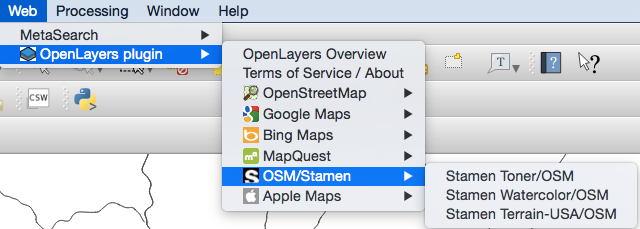
\includegraphics[width=0.25\textwidth]{figures/osmstatement}}
\caption{memilih basemap}
\label {osmstatement}
\end{figure}
\begin{enumerate}
\item
Klik menu Web, arahkan ke OpenLayers Plugin, arahkan ke OSM / Stamen, dan klik Stamen Toner / OSM. Ini menambahkan basemap hitam-putih dari data OpenStreetMap yang disediakan oleh Stamen .
\item
Jika basemap mengaburkan lapisan garis Anda, seret basemap ke bagian bawah daftar lapisan.
\end{enumerate}

Shapefiles dan GeoJSONs semuanya memiliki referensi spasial WGS 84, dan yang lebih spesifik lagi, EPSG: 4326. Saat menggunakan perangkat lunak GIS, seperti QGIS atau ArcMap, Anda harus bisa melapisi lapisan OSM dengan orang lain di peta Anda (perhatikan bahwa di QGIS, Anda perlu mengaktifkan proyeksi langsung di properti proyek). Jika Anda mengalami masalah dengan penyelarasan data, tinjau dokumentasi perangkat lunak yang Anda gunakan untuk mendapatkan petunjuk tentang pemecahan masalah.

\subsection{Lihat nilai atribut ekstrak}

Lapisan baris memiliki lebih dari 100.000 fitur di dalamnya, mewakili setiap baris di OSM di wilayah ini, walaupun Anda hanya tertarik untuk memetakan jalan untuk tutorial ini. Anda dapat melihat tabel atribut untuk memahami istilah pencarian yang akan digunakan untuk membatasi tampilan hanya pada fitur tertentu.
Di OSM, fitur dikenali melalui tag yang menggambarkan atribut sebagai kunci dan nilai. Kuncinya adalah kategori yang luas, seperti highway , dan nilainya memberikan rincian lebih lanjut, seperti jenis jalan atau namanya.
\begin{enumerate}
\item
Di bawah Lapisan, klik kanan layer sydney australia osm line dan klik Open Attribute Table.
\item
Di dalam tabel, kolom di bagian atas mewakili kunci yang paling umum.Baris adalah fitur individu di database OSM yang direferensikan oleh nomor identifikasi OSM mereka. Saat Anda melihat nilai atribut, perhatikan bahwa sebagian besar adalah NULL , yang menunjukkan bahwa tag belum terisi.

\begin{figure}[ht]
\centerline{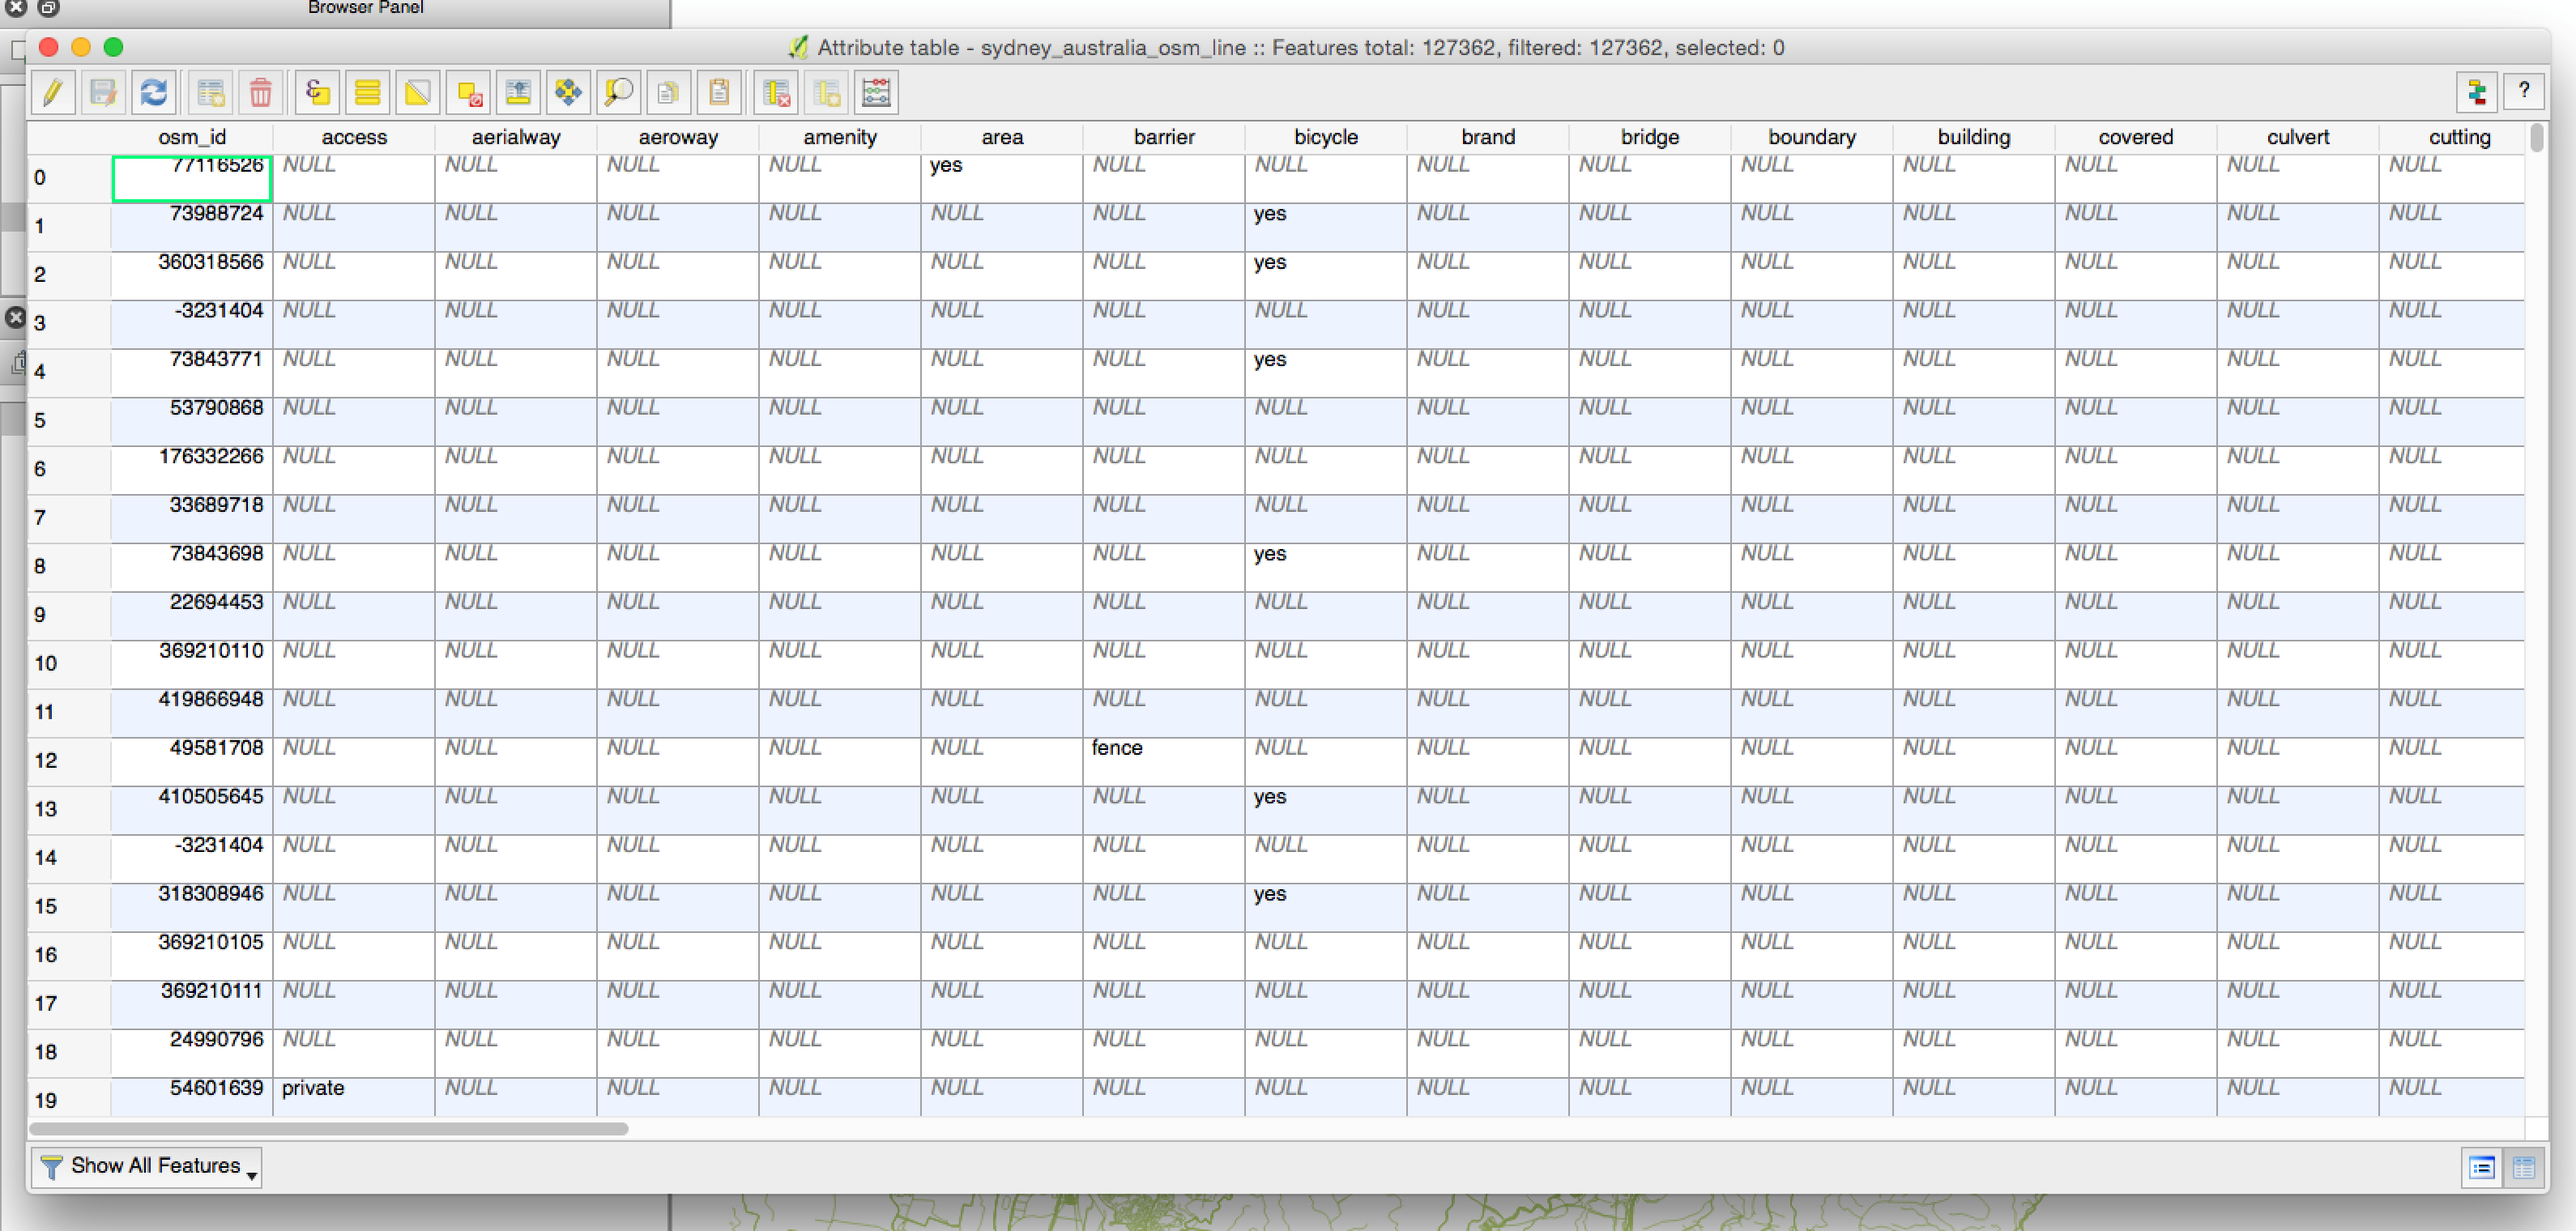
\includegraphics[width=0.25\textwidth]{figures/tabelosm}}
\caption{tabel database osm}
\label {tabelosm}
\end{figure}

 \item
Gulir ke kanan untuk melihat bidang jalan raya dan gulir ke bawah untuk melihat nilai di bidang itu.
\end{enumerate}

\subsection{Permintaan untuk fitur jalan}
Saat Anda melihat melalui meja, Anda mungkin telah memperhatikan beberapa fitur dengan nilai jalan tol . Jalan tol adalah jalan tertinggi di suatu wilayah. Anda dapat meminta tabel atribut untuk menampilkan hanya fitur yang diklasifikasikan sebagai jalan raya dekat Lisbon.
\begin{enumerate}
\item
Klik kanan layer dan klik Filter. Ini akan membuka kotak dialog di mana Anda dapat memasukkan kueri untuk memfilter lapisan.
\item
Di daftar Fields, klik dua kali highway untuk menambahkannya ke kotak ekspresi di bawah ini. Bidang adalah istilah lain untuk kolom di tabel atribut.
\item
Di bawah Operator, klik tombol equals .
\item
Di bawah Nilai, klik Semua untuk mendapatkan daftar nilai yang tersedia untuk bidang jalan raya.
\item
Klik dua kali motorway untuk menambahkannya ke ungkapan. Ekspresi Anda harus membaca: "highway" = 'motorway' .
 \item
Klik tombol Uji untuk memverifikasi sintaks kueri Anda. Anda harus menerima pesan yang menunjukkan bahwa lebih dari 1.000 baris telah dikembalikan. Jika tidak, pastikan teks Anda sesuai dengan teks pada gambar.
\item
Klik OK
\end{enumerate}

Tip: Dalam beberapa kasus, melakukan kueri di QGIS mungkin gagal jika shapefile memiliki periode atau titik pada namanya. Jika ini terjadi, ganti nama shapefile untuk menghapus periode. Anda seharusnya tidak melihat ini dengan Metro Extracts karena file-nya menggunakan underscore.

Tabel peta dan atribut sekarang menunjukkan lebih sedikit fitur karena hanya jalan raya yang ditampilkan. Fitur lain yang tidak memuaskan kueri masih ada di shapefile, tapi disembunyikan dari peta. Anda bisa mengekspor fitur, meski jika Anda ingin membuat layer baru hanya dengan jalur jalan tol. Jika Anda ingin menarik semua fitur lagi, Anda dapat menghapus kueri.
Kesederhanaan memiliki semua fitur garis yang dikelompokkan menjadi satu lapisan garis adalah keuntungan dari format osm2pgsql, namun memerlukan kueri kinerja untuk menjadi yang paling berguna.
Ubah simbol untuk fitur garis
Karena jalan raya adalah jalan utama, sebaiknya jalan raya diperlihatkan dengan garis tebal. QGIS hadir dengan serangkaian gaya yang sudah terisi.Anda bisa memilih untuk menggunakan salah satunya atau membangun simbol Anda sendiri untuk menampilkan jalan raya.
\begin{enumerate}
\item 
Di bawah Lapisan, klik dua kali lapisan garis untuk membuka propertinya.
\item
Klik tab Style.
\item
Temukan simbol Motorway dalam daftar gaya dan klik itu.
\item
Klik OK untuk menerapkan simbol.
\end{enumerate}
 
Karena setiap fitur baris diberikan secara individual, simbolnya tumpang tindih. Sebagai gantinya, garis harus digambar sebagai satu, fitur kontinyu.Anda bisa menggunakan teknik yang disebut simbol level drawing untuk menggabungkan batasan simbol.
\begin{enumerate}
\item
Buka kembali properti layer ke tab Styles.
\item
Klik tombol Advanced, dan klik Symbol levels.
\item
Centang Aktifkan tingkat simbol.
\item 
Klik OK pada semua kotak dialog.
\end{enumerate}

Perhatikan bahwa ada fungsi kartografi lainnya pada tab Styles untuk memperbaiki tampilan lapisan garis, termasuk transparansi. Anda bisa bereksperimen dengan ini sendiri.
Tambahkan file GeoJSON IMPOSM ke QGIS
Sejauh ini Anda telah menggunakan shapefile osm2pgsql, tapi Anda juga mendownload salah satu file GeoJSON yang tidak masuk akal. Selanjutnya, Anda akan menambahkan file itu ke QGIS.
Proses ekstraksi imposm menghasilkan serangkaian lapisan individu yang diberi nama oleh tema yang berbeda, seperti bangunan dan tempat. Anda juga dapat melihat file dengan -gen ditambahkan ke namanya, menunjukkan bahwa fitur telah digeneralisasi, atau disederhanakan. Karena fitur di lapisan imposm sudah dikategorikan berdasarkan atribut, kemungkinan besar Anda perlu menjalankan kueri Anda sendiri untuk menampilkan fitur yang Anda inginkan. Misalnya, jika ingin bekerja dengan jalan, Anda bisa menemukannya sudah dikelompokkan di lapisan jalan.
\begin{enumerate}
\item 
Pada panel Browser, buka folder sydney australia.imposm-geojson.
\item 
Tambahkan file sydney australia places GeoJSON ke peta.
\end{enumerate}

Dalam proses imposm, pengkategorian fitur ke lapisan tertentu ditentukan oleh daftar dan hierarki dalam file JSON . Dalam beberapa kasus, ini dapat menyebabkan tag OSM tertentu berada di beberapa bagian dari beberapa lapisan. Jika Anda tidak dapat menemukan nilai atribut tertentu di lapisan pertama yang Anda periksa, lihatlah file imposm lain, atau kembali dan ekspor dari lapisan osm2pgsql.
Ubah simbol untuk lapisan tempat
Fitur di lapisan tempat digambar dengan satu simbol, namun Anda dapat menggunakan nilai atribut untuk menggambarnya dalam kategori dengan simbol yang berbeda untuk nilai tertentu.
\begin{enumerate}
\item
Buka properti lapisan tempat.
\item
Klik tab Style.
\item
Di bawah Single Symbol, klik Categorized untuk mengubah metode menggambar untuk menggambar fitur berdasarkan kategori.
\item
Untuk Kolom, klik type untuk mengatur bidang type sebagai bidang yang berisi nilai yang akan digunakan untuk menggambar fitur.
\item
Klik Klasifikasikan di bawah kotak. Ini menambahkan semua nilai unik pada bidang jenis dan memberi mereka simbol yang terpisah.
\item
Jika ada simbol tanpa nilai atau entri legenda, sorotnya dalam daftar dan klik Delete.
\item
Untuk membuat simbol kota lebih besar dan lebih menonjol, klik kanan dalam daftar dan klik Change size. Atur ukuran menjadi 5.
\item
Anda bisa bereksperimen dengan warna dan ukuran simbol untuk membuat perbedaan poin tampak seperti yang Anda inginkan.
\item
Klik OK saat Anda selesai kembali ke peta dan melihat perubahan Anda.
\item
Opsional, simpan proyek Anda saat Anda selesai.
\end{enumerate}

Di luar QGIS di desktop, ada banyak alat berbasis web yang dapat Anda gunakan untuk menampilkan GeoJSON. Beberapa situs web yang bisa Anda gunakan tanpa scripting termasuk geojson.io dan situs GitHub . Tidak semua aplikasi mendukung sejumlah besar fitur atau pengeditan langsung GeoJSON, jadi Anda mungkin perlu mengkonversi ke format lain. Konsultasikan dokumentasi untuk perangkat lunak yang Anda gunakan untuk mempelajari lebih lanjut tentang kemampuan dan keterbatasannya.

\subsection{Ringkasan tutorial dan kota baru untuk Metro Extracts}
Dalam tutorial ini, Anda mendownload berbagai format file dari Metro Extracts, menambahkan lapisan ke QGIS, dan melakukan query dan mengatur simbol untuk fitur. Anda harus memiliki gagasan yang lebih baik tentang isi setiap unduhan sehingga Anda dapat memutuskan mana yang paling sesuai untuk proyek Anda. Untuk mempelajari cara membuat ekstrak ubahsuaian, ikuti tutorial ini.

\subsection{Memilih Format File di Metro Extract}
Setelah anda memilih Ekstrak Metro dari https://mapzen.com/data/metro-extracts/, ada beberapa jenis format file data spasial yang dapat
anda pilih. Gambar di bawah ini dapat menunjukkan berbagai pilihan yang tersedia untuk setiap Metro Extract. Ini berkisar dari data yang
mentah dan tidak diformat yang bagus untuk pengolahan data hingga data yang diatur agar teratur untuk digunakan dalam aplikasi perangkatlunak atau pemetaan web.

Metro Extracts menawarkan format file data ruang dalam lingkup data mentah agar lebih banyak diproses. 
Berikut ini adalah penjelasan singkat tentang tipe data: Format yang kurang diproses, seperti xml dan pbf, ditujukan untuk pengembang yang menjalankan dengan alat mereka sendiri pada data. 
Untuk sebagian besar alur kerja pembuatan map, shapefile atau GeoJSON bekerja dengan baik karena ini dapat ditambahkan secara langsung ke banyak aplikasi perangkat lunak. 
Jika Anda ingin menambahkan data ini ke peta web, GeoJSON lebih diutamakan. Semua shapefiles yang diekstrak dan GeoJSONs menggunakan EPSG: 4326 untuk proyeksi.

\subsection{Data split by geometri}
Dalam data split ini juga bekerja dengan format file OSM2PGSQL dapat memisahkan data OpenStreetMap dari Metro Extract menjadi tiga file: garis, titik, dan poligon. 
Hal ini juga dapat membuat fitur dalam menampilkan dengan geometri tertentu dengan sederhana, namun setiap fitur akan mencakup semua dari berbagai tag OSM. 

\subsection{Data split by OSM tags}
Dalam format file IMPOSM adalah format file paling rapi yang ditawarkan di Metro Extracts. 
Format ini dapat menghasilkan beberapa file, dipisahkan oleh tag OSM dan diurutkan menjadi tipe yang tersusun seperti:

Batas administratif
Aeroways
Fasilitas
Bangunan
Penggunaan lahan
Tempat
Jalan
Daerah transportasi
Daerah Air
Jalan air

Penamaan untuk lapisan ini berasal langsung dari OpenStreetMap dan mungkin membingungkan jika Anda tidak terbiasa dengan tag OSM.
Berikut informasi lebih lanjut tentang bagaimana tag bekerja: http://wiki.openstreetmap.org/wiki/Map\_Features.

